\documentclass{beamer}

\usetheme{Warsaw}

\title{Uppaal. The Model Checker.}
\author{Patryk Kiepas}
\date{\today}

\begin{document}
%-------------------------------------------------------------------------
\begin{frame}
	\titlepage
\end{frame}

%-------------------------------------------------------------------------	
\section*{Outline}
\begin{frame}
	\tableofcontents
\end{frame}

%%%%%%%%%%%%%%%%%%%%%%%%%%%%%%%%%%%%%%%%%%%%%%%%%%%%%%%%%%%%%%%%%%%%%%%%%%
\section{Intro}
%%%%%%%%%%%%%%%%%%%%%%%%%%%%%%%%%%%%%%%%%%%%%%%%%%%%%%%%%%%%%%%%%%%%%%%%%%
\subsection{Quick look}
%-------------------------------------------------------------------------
\begin{frame}{Uppaal. What is it?}
	Uppaal is a model checker for real-time systems (in mind of embedded systems). What we can do with it?
	
	\begin{enumerate}
		\item Modeling
		\item Simulation
		\item Verification
	\end{enumerate}
	
	Internal representation of model consists of:
	
	\begin{itemize}
		\item Network of timed automata
		\item Extended with data types
	\end{itemize}

\end{frame}

\begin{frame}{Where to use?}
	``Any system can be analysed using a model checker, as long as it has \textit{states} and \textit{transitions} between states'' (from Chapter 1: A First Introduction to Uppaal by Frits Vaandrager) \newline
	
	Reactive systems such as:
	\begin{itemize}
		\item Hardware components
		\item Embedded controllers
		\item Network protocols
		\item Others...
	\end{itemize}
	Whenever there is need to handle real-time issues (the timing of transitions).
	
\end{frame}

\subsection{History}
%-------------------------------------------------------------------------
\begin{frame}{Brief history}
	Uppaal was started by Uppsala University, Sweden and Aalborg University, Denmark.
	
	Time-line of development:
	\begin{itemize}
		\item 1995 - project started
		\item 1999 - first beta
		\item 1999/2000 - first stable release (v 3.0.X)
		\item September 27, 2010 - latest stable release (v 4.0.13)
		\item July 1, 2014 - preview release (v 4.1.19)
	\end{itemize}
	
\end{frame}

\subsection{Versions}
\begin{frame}{Uppaal variations}
	Versions: Windows, Mac, Linux, 32/64 bits
	
	Available licenses:
	\begin{itemize}
		\item Academic use (more info: \href{http://www.uppaal.org/}{http://www.uppaal.org/})
		\item Commercial use (more info: \href{http://www.uppaal.com/}{http://www.uppaal.com/})
	\end{itemize}
\end{frame}

%%%%%%%%%%%%%%%%%%%%%%%%%%%%%%%%%%%%%%%%%%%%%%%%%%%%%%%%%%%%%%%%%%%%%%%%%%	
\section{The tool}
%%%%%%%%%%%%%%%%%%%%%%%%%%%%%%%%%%%%%%%%%%%%%%%%%%%%%%%%%%%%%%%%%%%%%%%%%%
\subsection{Uppaal GUI}
%%%%%%%%%%%%%%%%%%%%%%%%%%%%%%%%%%%%%%%%%%%%%%%%%%%%%%%%%%%%%%%%%%%%%%%%%%
\begin{frame}{Uppaal GUI - Main parts}
\vspace{-10mm}
\begin{columns}
	\begin{column}{0.8\textwidth}
		\begin{figure}[H]
			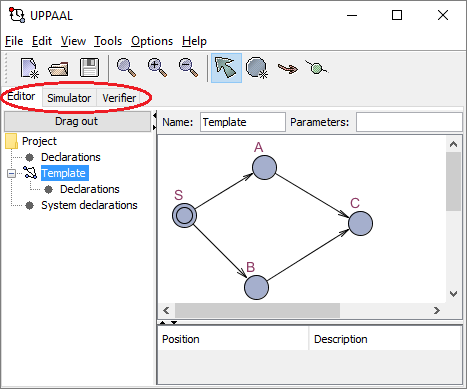
\includegraphics[scale=0.7]{img/uppaal_gui_small_editor.png}
		\end{figure}
	\end{column}
	
	\begin{column}{0.3\textwidth}
		\begin{itemize}
			\item System editor
			\item Simulator
			\item Verifier
		\end{itemize}
	\end{column}
\end{columns}		
\end{frame}

\begin{frame}{Uppaal GUI - System editor}
	\vspace{-10mm}
	\begin{columns}
		\begin{column}{0.8\textwidth}
			\begin{figure}[H]
				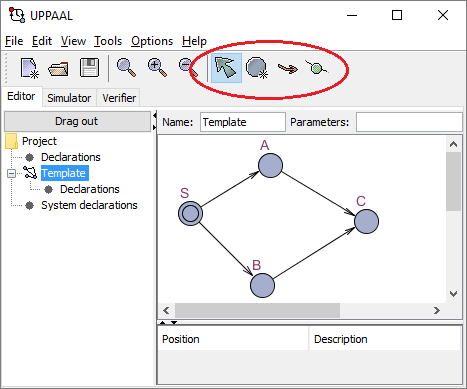
\includegraphics[scale=0.7]{img/uppaal_gui_small_editor_control.png}
			\end{figure}
		\end{column}
		
		\begin{column}{0.3\textwidth}
			\begin{itemize}
				\item Name: Template (default)
				\item Select
				\item Add location
				\item Add edge
				\item Add nail
				\item Syntax check (for global, local, system declarations)
			\end{itemize}
		\end{column}
	\end{columns}		
\end{frame}

\begin{frame}{Uppaal GUI - Simulator}
	\vspace{-5mm}
	\begin{columns}
		\begin{column}{0.8\textwidth}
			\begin{figure}[H]
				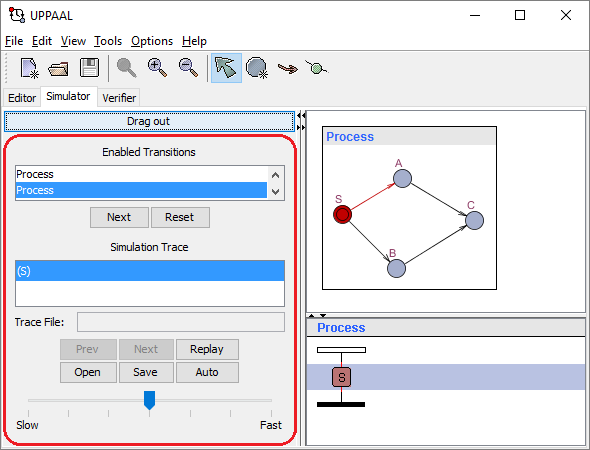
\includegraphics[scale=0.55]{img/uppaal_gui_small_simulation.png}
			\end{figure}
		\end{column}
		
		\begin{column}{0.35\textwidth}
			\begin{itemize}
				\item Select transition
				\item Track simulation
				\item Control (Prev/Next/Auto)
				\item Visualization
			\end{itemize}
		\end{column}
	\end{columns}		
\end{frame}

\begin{frame}{Uppaal GUI - Verifier}
	\vspace{-5mm}
	\begin{columns}
		\begin{column}{0.8\textwidth}
			\begin{figure}[H]
				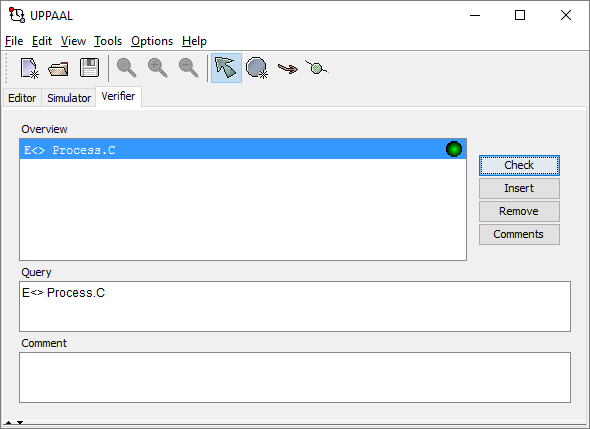
\includegraphics[scale=0.55]{img/uppaal_gui_small_verification.png}
			\end{figure}
		\end{column}
		
		\begin{column}{0.35\textwidth}
			\begin{itemize}
				\item Query editor
				\item Check query
				\item Overview
				\item Save/load
			\end{itemize}
		\end{column}
	\end{columns}		
\end{frame}

%%%%%%%%%%%%%%%%%%%%%%%%%%%%%%%%%%%%%%%%%%%%%%%%%%%%%%%%%%%%%%%%%%%%%%%%%%	
\subsection{Model structure}
%%%%%%%%%%%%%%%%%%%%%%%%%%%%%%%%%%%%%%%%%%%%%%%%%%%%%%%%%%%%%%%%%%%%%%%%%%
\begin{frame}{System/model/project}
%We build so called system/model/project.
	
	\begin{columns}
		\begin{column}{0.7\textwidth}
			Description of system consist of:	
			\begin{itemize}
				\item Concurrent process templates modelled using timed-automata (here \textit{P0} and \textit{P1});
				\item Local declarations for each process;
				\item Global declarations for whole system;
				\item System definition.
			\end{itemize}
		\end{column}
		
		\begin{column}{0.37\textwidth}
			\begin{figure}[H]
				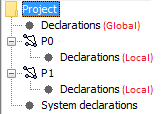
\includegraphics[scale=1]{img/uppaal_project.png}
			\end{figure}
		\end{column}
	\end{columns}
\end{frame}

\begin{frame}{Process/automata}
	
	Process is a timed-automata represent as diagram with states
	(called locations) and transitions between states (called edges). Timed-automata is finite state machine with time (clocks).\newline

	Each process has only one \textbf{initial location}.\newline
	
	Processes execute concurrently and they can be synchronized using channels.\newline
\end{frame}

\begin{frame}{Time/clocks}
	Time is continuous and the clocks measure time progress. Time progress globally and clocks values increase at the same rate for the whole system.\newline
	
	A clock is a special type of variable with domain being a set of non-negative real numbers. At system start, all clocks have value 0.\newline
	
	Using clocks we can specify:
	\begin{itemize}
		\item \textbf{Invariants} - upper bounds on timing, describes how long we can stay in given \textit{location};
		\item \textbf{Guard} - lower bound on timing, describes after what amount of time a \textit{transition} can be executed.
	\end{itemize}
	
	We can test the value of clock using standard expressions or we can reset clock.
\end{frame}

\begin{frame}{Location/state (part I)}
	\begin{figure}[H]
		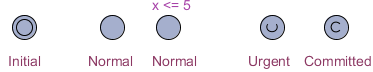
\includegraphics[scale=1]{img/uppaal_locations.png}
	\end{figure}
	
	Location represents state of the system. There are four types of locations:
	\begin{itemize}
		\item Initial (one for each process);
		\item Normal (with or without \textbf{invariants});
		\item Urgent (time cannot elapse in this location, so transition to another location must occur \textbf{immediately});
		\item Committed.
	\end{itemize}
\end{frame}

\begin{frame}{Location/state (part II)}
		\begin{figure}[H]
			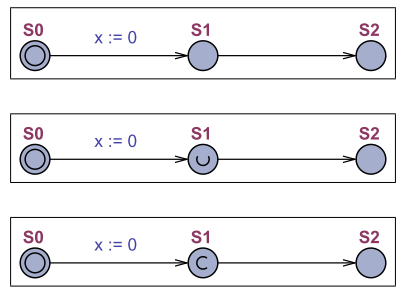
\includegraphics[scale=0.8]{img/todo_location_types.png}
		\end{figure}
\end{frame}

\begin{frame}{Edge/transition (part I)}
	An edge/transition connects two locations. Edges can have four types of annotations:
	
	\begin{itemize}
		\item \textbf{Selection} - binds a given identifier to a value in a scope of current transition; allowed types: \textit{boundend integers}, \textit{scalar sets}; defined here identifiers will shadow local/global variables.
		\item \textbf{Guard} - transition is enabled only if guard's expression evaluates to \textbf{true} and consists of:
		\begin{itemize}
			\item Conjunction of simple conditions on clocks;
			\item Differences between clocks;
			\item Boolean expressions not involving clocks.
		\end{itemize}
		\item \textbf{Synchronization} - transition labelled with complementary actions (e.g. \textit{a!} and \textit{a?}) will synchronize over a common channel (here channel \textit{a})
	\end{itemize}
	%Now, remove the invariant and change the guard to x >= 2 and x <= 3. As you can see the system may take the same transitions as before, but there is now a deadlock: the system may be stuck if it does not take the transition after 3 time units.
	
\end{frame}

\begin{frame}{Edge/transition (part II)}
	\begin{itemize}
		\item \textbf{Update} - evaluate given expression when transition occur.
	\end{itemize}	
	
	\begin{figure}[H]
		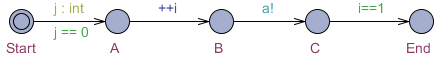
\includegraphics[scale=0.8]{img/uppaal_transitions.png}
	\end{figure}
	Example of transitions with annotations:
	\begin{itemize}
		\item Selection: \textit{j : int};
		\item Update: \textit{++i};
		\item Synchronization: \textit{a!};
		\item Guard: \textit{j==0}, \textit{i==1}.
	\end{itemize}
\end{frame}

\begin{frame}{Edge/transition (part III)}
	Without prior specification, all transitions occur instantaneously and do not take time.\newline
	
	When no further transition is possible we reach so called \textbf{deadlock state}.\newline
	
	Unspecified choice is called non-deterministic:\newline
	\vspace{-8mm}
	\begin{columns}
		\begin{column}{.5\textwidth}
			\begin{figure}[H]
				\label{img:ndc}
				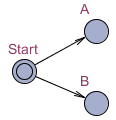
\includegraphics[scale=0.7]{img/uppaal_non_deterministic_choice.png}
				\caption{Non-deterministic choice.}
			\end{figure}
		\end{column}
		\begin{column}{.5\textwidth}
			\begin{figure}[H]
				\label{img:dc}
				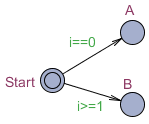
\includegraphics[scale=0.7]{img/uppaal_deterministic_choice.png}
				\caption{Deterministic choice.}
			\end{figure}
		\end{column}		
	\end{columns}
\end{frame}

\begin{frame}{Parameters}
	
	Template of process can have parameters with different call semantics (C++ syntax):
	
	\begin{itemize}
		\item call-by-value (using local copy, e.g. \textit{int a})
		\item call-by-reference (using original value, e.g. \textit{int\& a})
	\end{itemize}
	
	Clocks and channels must always be call-by-reference parameters.
	Uppaal does not allow data parameters for synchronization channels (?).
	
	In template parameters field: urgent chan \&get, chan \&put.
	When creating templates:
	Hammer = Tool(get\_hammer, put\_hammer);
	Mallet = Tool(get\_mallet, put\_mallet);
\end{frame}

\begin{frame}{System declaration}
	
\end{frame}

\begin{frame}{Channels}
	(!)  Uppaal offers urgent channels (defined using urgent chan) that are synchronization that must be taken when the transition is enabled, without delay. Clock conditions on these transitions are not allowed.
	
	(!) There is no value passing through the channels
	
	(!)The synchronization mechanism in Uppaal is a hand-shaking synchronization: two processes take a transition at the same time, one will have an a! and the other an a?, with a being the synchronization channel. When taking a transition, two actions are possible: assignment of variables or reset of clocks. 
	
	Uppaal does not allow
	data parameters for synchronization channels.
	
	When a synchronization channel is urgent, this means that whenever a synchronization with this channel is enabled, time can not advance and a transition has to be taken immediately.\newline
	
	In order to model the synchronization between tools and jobbers,
	we use the notion of (synchronization) channels from Uppaal. Once “a” has been
	declared as a channel, transitions can be labelled with either a! or a?. This can be
	done by double clicking (within the Editor) transitions with the Select tool, and then
	writing a! or a? in the Sync field. When two automata synchronize on channel “a”,
	this means that an a! transition of one automaton occurs simultaneously with an
	a? transition of another automaton. An a! or a? transition can never occur on its
	own: a! always has to synchronize with a?, and vice versa. If there is one automaton
	S that can do an a! but two automata R1 and R2 that can do an a?, then there is
	a non-deterministic choice and S can synchronize with either R1 or R2. The other
	automaton has do something else or has to wait until the next a! synchronization
	will be offered.
\end{frame}

\begin{frame}{Variables}
	Global/local variables\newline
	
	Examples:\newline
	
	$\text{const int } J = 10;$\\
	$ int[0,J] \text{ jobs}; // \text{ integer with min. value 0 and max. value J}$\newline
	
	The domain of integer is always bounded. By default $int$ has range $[-32768, 32768]$.\newline
	
	Variable assigned with a value outside of its domain generates ``run-time error''.\newline
	
	Transition can have guards: expressions which use variables. Every transition have guard, by default they return \textbf{true}.\newline
	
	Uppaal does not support enumerated types.\newline
	*
	Arrays: const int[0,2] jobs[J] = {H,A,H,H,H,E,E,A,A,A};
\end{frame}

\begin{frame}{Expressions with variables}
	All are C-like:
	\begin{itemize}
		\item jobs++
		\item jobs = jobs + 1
		\item jobs := jobs + 1
	\end{itemize}
	
\end{frame}

\begin{frame}{Verification}
	
	Whereas the Verifier has an option to compute the fastest execution leading to
	a certain state, there is no corresponding option to compute the slowest execution.
\end{frame}

\begin{frame}{Queries (part I)}	
	Query is a property expressed as temporal logic formula, that may or may not hold for a given model. The Verifier can establish whether a Query is \textbf{satisfied} or \textbf{not}.\newline
	Basic queries:
	\begin{itemize}
		\item \textit{A[] p} : for all paths \textit{p} \textbf{always holds};
		\item \textit{E[] p} : there exists a path where \textit{p} \textbf{always holds};		
		\item \textit{A$<>$ p} : for all paths \textit{p} will \textbf{eventually hold};
		\item \textit{E$<>$ p} : there exists a path where \textit{p} \textbf{eventually holds};
		\item \textit{p --$>$ q} : whenever p holds q will eventually hold.

	\end{itemize}
	
	Simple queries are in form of e.g \textit{A[] p} where \textit{p} is an expression build from \textbf{boolean combination} of \textbf{atomic propositions}.
\end{frame}

\begin{frame}{Queries (part II)}
	The simplest atomic proposition can be of the form \textit{P0.C}, where \textit{P0} is an automaton and \textit{C} is a location. Such a proposition is \textbf{true} if process \textit{P0} is in location \textit{C}.\newline
	
	\begin{tabular}{|c|c|c|}
		\hline \textbf{Expression} & \textbf{Name} & \textbf{True when...} \\ 
		\hline $e\text{ }\&\&\text{ }f$ & and & $e$ and $f$ evaluate to \textbf{true}	 \\ 
		\hline $e\text{ }||\text{ }f$ & or & $e$ or $f$ evaluate to \textbf{true} \\ 
		\hline $e\text{ }==\text{ }f$ & equality & $e$ and $f$ evaluate to the same value \\ 
		\hline $e\text{ }imply\text{ }f$ & implication & $e$ evaluate to \textbf{false} or $f$ evaluate to \textbf{true}\\ 
		\hline $e\text{ }not\text{ }f$ & negation & $e$ evaluates to \textbf{false} \\ 
		\hline 
	\end{tabular} 

\end{frame}

\begin{frame}{Queries (part III)}
	\begin{itemize}
		\item $A[] \text{ not deadlock}$
		\item $E<> \text{Process\_1.C}$
		\item $E<> (\text{Process\_1.C } \&\& \text{ Process\_2.C})$
		\item $A[] \text{ now } >= \text{ 200 imply }$
		$(\text{Belt.end } \&\& \text{ Jobber1.begin } \&\& \text{Jobber2.begin})$
		\item $A[] \text{ Obs.taken imply } (x>=2 \text{ and } x<=3)$
		\item $E<> \text{ Obs.idle and } x>2$
		\item $A[] \text{ Obs.idle imply } x<=3$
		
	\end{itemize}
\end{frame}

\begin{frame}{Reasoning}
	(!)The tool just uses brute force to explore all the reachable global states of the model and to check for each of these	states whether both jobbers are working on a hard job.
	
	
	(!)Model checker engine. It can run in server mode on a more powerful, dedicated machine.

	(!) 
	More precisely, the engine uses on-the-fly verification combined with a symbolic technique reducing the verification problem to that of solving simple constraint systems [YPD94, LPY95]. The
	verifier checks for simple invariants and reachability properties for efficiency reasons. Other properties may be checked by using testing automata [JLS96] or the decorated system with debugging
	information [LPY97].
	
	(!)Then we can ask the verifier to check reachability properties, i.e., if a certain
	state is reachable or not. This is called model-checking and it is basically an exhaustive search
	that covers all possible dynamic behaviours of the system.
\end{frame}

\begin{frame}{Diagnostic traces}
	
	(!)Uppaal can also provide a concrete example that illustrates why the property holds (for $E<>$ properties) or not (for $A[]$ properties, so called: \textit{counterexample}).\newline
	
	(!)In the case of $E<>$ properties that do not hold, or $A[]$ properties that hold, Uppaal can only report that it exhaustively checked all the reachable states of the model and didn’t find anything.\newline
	
	(!)We choose under \textit{Options} the entry \textit{Diagnostic Trace} and then select the option \textit{Shortest}. Simulator will then show found diagnostic trace.
\end{frame}

\begin{frame}{Saving data}
	We can save various types of data:
	
	\begin{itemize}
		\item Model/system - \textit{*.xml} file;
		\item Queries - \textit{*.q} file;
		\item Traces (binary) - \textit{*.xtr} file.
	\end{itemize}
\end{frame}

\begin{frame}{Keeping models manageable}
	\begin{itemize}
		\item Committed locations - reduce significantly the state space, but on the other hand they can take away relevant states;
		\item Variables and its ranges - use small amount of variables with the shortest value ranges;
		\item Clocks - has an important impact on the complexity of the model.
	\end{itemize}
\end{frame}

%%%%%%%%%%%%%%%%%%%%%%%%%%%%%%%%%%%%%%%%%%%%%%%%%%%%%%%%%%%%%%%%%%%%%%%%%%	
\section{Example}
%%%%%%%%%%%%%%%%%%%%%%%%%%%%%%%%%%%%%%%%%%%%%%%%%%%%%%%%%%%%%%%%%%%%%%%%%%

\begin{frame}{Examples}
	\begin{enumerate}
		\item First automata, deterministic and non-deterministic choices.
		\item Location types.
		\item Simple synchronization.
		\item Guards and invariants.
		\item BIG! Production line.
	\end{enumerate}
\end{frame}

%%%%%%%%%%%%%%%%%%%%%%%%%%%%%%%%%%%%%%%%%%%%%%%%%%%%%%%%%%%%%%%%%%%%%%%%%%	
\section{Bibliography}
%%%%%%%%%%%%%%%%%%%%%%%%%%%%%%%%%%%%%%%%%%%%%%%%%%%%%%%%%%%%%%%%%%%%%%%%%%

\begin{frame}
	\begin{itemize}
		\item F.W. Vaandrager. \textit{``A First Introduction to Uppaal''} In J. Tretmans, editor. Quasimodo Handbook. To appear.
		\item \textit{Uppaal 4.0: Small Tutorial. A short description of the tool as well as some examples.}
		\item \textit{Uppaal Help/Documentation}. Built-in. Uppaal 4.0.14, May 2014.
	\end{itemize}
\end{frame}

\end{document}
